\documentclass[12pt,]{article}
\usepackage[T1]{fontenc}
\usepackage{lmodern}
\usepackage{amssymb,amsmath}
\usepackage{ifxetex,ifluatex}
\usepackage{fixltx2e} % provides \textsubscript
% use upquote if available, for straight quotes in verbatim environments
\IfFileExists{upquote.sty}{\usepackage{upquote}}{}
\ifnum 0\ifxetex 1\fi\ifluatex 1\fi=0 % if pdftex
  \usepackage[utf8]{inputenc}
\else % if luatex or xelatex
  \ifxetex
    \usepackage{mathspec}
    \usepackage{xltxtra,xunicode}
  \else
    \usepackage{fontspec}
  \fi
  \defaultfontfeatures{Mapping=tex-text,Scale=MatchLowercase}
  \newcommand{\euro}{€}
\fi
% use microtype if available
\IfFileExists{microtype.sty}{\usepackage{microtype}}{}
\usepackage[margin=1in]{geometry}
\usepackage{graphicx}
% Redefine \includegraphics so that, unless explicit options are
% given, the image width will not exceed the width of the page.
% Images get their normal width if they fit onto the page, but
% are scaled down if they would overflow the margins.
\makeatletter
\def\ScaleIfNeeded{%
  \ifdim\Gin@nat@width>\linewidth
    \linewidth
  \else
    \Gin@nat@width
  \fi
}
\makeatother
\let\Oldincludegraphics\includegraphics
{%
 \catcode`\@=11\relax%
 \gdef\includegraphics{\@ifnextchar[{\Oldincludegraphics}{\Oldincludegraphics[width=\ScaleIfNeeded]}}%
}%
\ifxetex
  \usepackage[setpagesize=false, % page size defined by xetex
              unicode=false, % unicode breaks when used with xetex
              xetex]{hyperref}
\else
  \usepackage[unicode=true]{hyperref}
\fi
\hypersetup{breaklinks=true,
            bookmarks=true,
            pdfauthor={},
            pdftitle={},
            colorlinks=true,
            citecolor=blue,
            urlcolor=blue,
            linkcolor=magenta,
            pdfborder={0 0 0}}
\urlstyle{same}  % don't use monospace font for urls
\setlength{\parindent}{0pt}
\setlength{\parskip}{6pt plus 2pt minus 1pt}
\setlength{\emergencystretch}{3em}  % prevent overfull lines
\setcounter{secnumdepth}{0}

\author{}
\date{}
\usepackage{lineno}
\linenumbers
\usepackage{setspace}
\doublespacing
\usepackage{todonotes}

\begin{document}

\normalsize


\section{Comparing IPM with approximate demographic stochasticity to
IBM}\label{comparing-ipm-with-approximate-demographic-stochasticity-to-ibm}

Our approach to incorporating demographic stochasticity in integral
projection models (IPMs) is new, and thus requires testing.
Individually-based models (IBMs) inherently include demographic
stochasticity (e.g., ``coin flips'' for survival of a genet from a
Bernoulli trial). IBMs, then, provide the baseline against which to
compare an IPM with our approximation to demogrpahic stochasticity. If
the two models produce similar equilibrium cover and species synchrony,
then we can conclude our approximation is valid. Here we use the Idaho
dataset as a test case, and simulate communities from the IPM with
demographic stochastisticy and the IBM. We ignore temporal variation due
to random year effects to isolate variation from demographic
stochasticity alone.

Figure 1 compares the distribution of percent cover over 2,000
iterations (after a 500 iteration burn in) for each species from the IBM
and the IPM with approximate demographic stochasticity. There are some
small differences, but overall the approximation leads to similar long
term population dynamics when compared to the IBM. The IPM and IBM also
show similar interannual dynamics, as signified by the very similar
synchrony metrics (Table 1). Moreover, species synchrony from models
where only demographic stochasticity is acting matches theoretical
expectations: theory predicts synchrony = 1/\emph{S} (where \emph{S} is
species richness) when demographic stochasticity is much stronger than
the effects of environmental stochasticity and species interactions.
Indeed, the IPM produces synchrony = 0.3 (1/3 with 3 species) when we
exclude random year effects (species interactions are present, but not
influential due to small competition coefficients).

\begin{figure}[htbp]
\centering
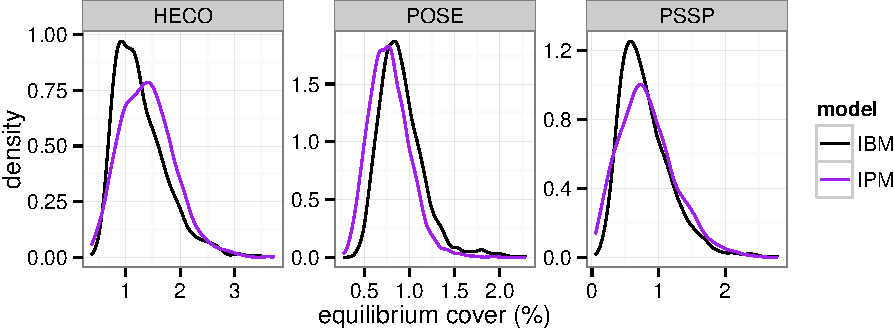
\includegraphics{./demog_stoch_test_files/figure-latex/figs.pdf}
\caption{Density estimates of equilibrium cover from 2,000 iterations
from each model.}
\end{figure}

\begin{table}[ht]
\centering
\caption{Species synchrony of percent cover and per capita growth rates.} 
\begin{tabular}{lrr}
  \hline
Model & Cover Sychrony & Growth Rate Synchrony \\ 
  \hline
IPM & 0.33 & 0.34 \\ 
  IBM & 0.34 & 0.33 \\ 
   \hline
\end{tabular}
\end{table}

\end{document}
